\documentclass[12pt, a4paper]{scrartcl}

%used packages
\usepackage[utf8]{inputenc}
\usepackage[ngerman]{babel}
\usepackage{xcolor}
\usepackage{graphicx}
\usepackage{hyperref}
\usepackage{makecell}
\usepackage{sectsty}
\usepackage{blindtext}

\usepackage{tabularx}
\usepackage{eurosym}
\usepackage{caption}
\usepackage{subcaption}


\usepackage{fancyhdr}
\pagestyle{fancy}
\renewcommand{\sectionmark}[1]{\markright{#1}}
\renewcommand{\footrulewidth}{0.4pt}
\fancyhead{}
\fancyhead[R]{\rightmark}
\fancyfoot{}
\fancyfoot[R]{\thepage}


%costum commads
\newcommand{\mailto}[1]{\href{mailto:#1}{\color{silver}{#1}}}
\newcommand{\NameMail}[2]{{{#1}}\\{\small\mailto{#2}}}
\newcommand{\mysubsection}[1]{\subsection*{#1}
	\addcontentsline{toc}{subsection}{#1}}

%color scheme
\definecolor{spaceCadet}{HTML}{2D3142}
\definecolor{independence}{HTML}{4F5F75}
\definecolor{silver}{HTML}{BFC0C0}
\definecolor{tumbleweed}{HTML}{D7A28A}
\definecolor{mandarin}{HTML}{EF8354}
\definecolor{sinopia}{HTML}{D12911}

%hyperref setup
\hypersetup{
	colorlinks,
	linkcolor=sinopia,
	citecolor={blue!50!black},
	urlcolor={sinopia!80!black}
}

%editig section and subsection style
\sectionfont{\color{spaceCadet}}
\subsectionfont{\color{independence}}
\subsubsectionfont{\color{tumbleweed}}

\begin{document}
	\begin{titlepage}
		\raggedleft
		
		\textcolor{mandarin}{\rule{1pt}{\textheight}} 
		\hspace{0.05\textwidth}
		\parbox[b]{0.85\textwidth}{
			
			{\Huge\bfseries \textcolor{spaceCadet}{Smart Mirror}}\\[1\baselineskip]
			{\LARGE \bfseries \textcolor{independence}{Fakultät Informatik Mathematik}}\\[1\baselineskip]
			{\Large  \textcolor{independence}{OTH Regensburg}}\\[1\baselineskip]
			{\large \textcolor{independence}{Human Computer Interaction}}\\[2\baselineskip]
			
			
			
			
			{\LARGE\bfseries\textcolor{spaceCadet}{Projektbericht}}\\[0.2\baselineskip]
			{\Large\textcolor{independence}{Wintersemester 2020/2021}} \\[0.2\baselineskip]
			{\textcolor{independence}{\noindent 12. Februar 2021}} \\[3\baselineskip]
			
			\vspace{0.4\textheight}
			\begin{tabular}{ c c }
				\makecell[l]{\NameMail{Patrick Gruber}{patrick.gruber@st.oth-regensburg.de}}
				& \makecell[l]{\NameMail{Tobias Gubo}{tobias1.gubo@st.oth-regensburg.de}}\\
				\makecell[l]{\NameMail{Michael Lazik}{michael1.lazik@st.oth-regensburg.de}} 
				& \makecell[l]{\NameMail{Marcus Müller}{marcus.mueller@st.oth-regensburg.de}}
			\end{tabular}\\ [2\baselineskip]
		}
		
	\end{titlepage}
	
	\tableofcontents
	\thispagestyle{empty}
	\pagebreak
	\setcounter{page}{1}
	
	\section{Projektplanung}
	\begin{quote}
		{Nur wer sein Ziel kennt, findet den Weg.} - Laozi
	\end{quote}
	Wie jedes gute Projekt beginnt man mit der grundlegenden Planung und Strukturierung 
	\subsection{Festlegen der Resourcen}
	Der erste und elementarste Schritt war es sich zu überlegen, wie ein Produkt wie der Smart Mirror überhaupt realisiert werden kann. Dafür haben wir uns im Internet auf die Suche gemacht und sind dort an mehreren Stellen auf DIY-Projekte gestoßen, die eine ähnliche Idee umgesetzt haben. Die fundamentalen Bestandteile waren jedoch oft sehr vergleichbar. Man benötigt einen Einwegspiegel, der das Licht von einer Seite durchlässt und von der anderen Seite verspiegelt ist. Mit einem LED-Display hinter der Spiegelscheibe lässt sich so eine Anzeigefläche erschaffen, die für den Betrachter nur sichtbar ist, wenn sie beleuchtet ist. Die Art und Weise, wie das Display angesprochen wird ist wieder eine freiere Entscheidung. Wir haben uns dafür entschieden einen RaspberryPi 3b zu verwenden. Dies hat mehrere Gründe, die im Laufe des Berichts noch genauer beleuchtet werden. Montiert wird das Spiegeldisplay in einem Rahmen aus Holz, um ein einheitliches Erscheinungsbild zu kreieren. Als letztes wichtiges Element ist noch der LeapMotion-Controller zu nennen, der eine einfache Möglichkeit bildet, um die Gestik des Nutzers zu erkennen, um somit die Interaktion zwischen Mensch und Maschine zu ermöglichen.
	\subsubsection*{Grobe Kostenaufstellung}
	\begin{tabularx}{0.95\textwidth}{|X|l|r|}
		\hline
		\textcolor{tumbleweed}{\underline{\textbf{Name}}} & \textcolor{tumbleweed}{\underline{\textbf{Zulieferer}}} & \textcolor{tumbleweed}{\underline{\textbf{Preis}}}\\
		\hline
		Spiegelglas 70x100cm & GlasStar&ca. 125\euro\\
		\hline
		Display 17" mit Controller & Amazon & ca. 160\euro\\
		\hline
		LeapMotion Controller & AdaFruit & ca. 100\euro \\
		\hline
		Holzrahmen 70x100cm & Amazon & ca. 50\euro\\
		\hline
		Raspberry Pi & Amazon & ca. 40\euro\\
		\hline
		Kabel und Verbidungen & Amazin & ca. 50\euro\\
		\hline
		\textcolor{tumbleweed}{\textbf{Gesamt}}& & \textbf{ca. 525\euro}\\
		\hline
	\end{tabularx}

	\newpage
	
	\section{Verstehen und Festlegen des Nutzungskontexts}
	Nachdem die Ressourcen festgelegt worden sind, musste der Nutzungskontext definiert, verstanden und festgelegt werden. Hierbei wurde überlegt, wer die Benutzer sind und wie diese mit dem Smart Mirror interagieren werden.
	\subsection{Beschreibung des Nutzungskontexts}
	Unsere primären Benutzer sind die Probanden, die den Smart Mirror testen und damit Daten zur Auswertung liefern.\\
	Die sekundären Benutzer sind die Mitglieder des Projektteams, die auf Basis der gewonnen Daten den Smart Mirror weiter entwickeln.\\
	Mit dem Smart Mirror sollen den Benutzern innerhalb kürzester Zeit die wichtigsten Informationen gezeigt bekommen.\\
	Dabei soll dem Benutzer gezeigt werden:
	\begin{itemize}
		\setlength\itemsep{-0.5em}
		\item Uhrzeit
		\item Wetter (Uhrzeitbedingt)
		\item RSS-Feed
	\end{itemize}
	Zudem kann der Benutzer individuelle Informationen anzeigen lassen. In unserem Projekt sind das:
	\begin{itemize}
		\setlength\itemsep{-0.5em}
		\item Termine
		\item  ToDo-Liste
		\item Fahrzeiten ÖPNV
		\item Verkehrslage
		\item Speißeplan
	\end{itemize}
	Für den Smart Mirror benötigt der Nutzer keine Ausrüstung. Sie müssen nur wissen, wie man mit dem Smart Mirror interagiert und wie man durch den Pageflow die Seiten wechselt. Der Smart Mirror kann an jeden von den Benutzern beliebig ausgewählten Ort stehen. Das Projektteam hat sich jedoch auf das Schlafzimmer als Örtlichkeit für den Smart Mirror festgelegt.\\
	Damit der Nutzungskontext aus Sicht der primären Benutzer verstanden werden kann, wurden Interviews mit den Probanden durchgeführt.
	Dabei wurden vor allem zu Beginn möglichst offene, neutrale und allgemeine Fragen gestellt, also das "Warum?", die dann immer mehr in die Materie des Smart Mirrors gingen, also das "Wie?". Hier konnten die Probanden uns ihre Vorstellung eines Smart Mirrors offenbaren und das Projektteam konnte anhand dieser Informationen die Nutzungsanforderungen festlegen. 
	
	\newpage
	
	\section{Erarbeitung von Gestaltungslösungen zur Erfüllung des Nutzungskontexts}
	\subsection{Erstellen der Interaktionsspezifikation}
	Anhand der zuvor, durch Umfragen und Formulare erlangten Informationen über das potentielle Nutzungsverhaltens der User, wurden nun die möglichen Varianten der Interaktion mit dem Spiegel validiert.\\
	Dabei wurden folgende Optionen betrachtet:
	\begin{itemize}
		\setlength\itemsep{-0.5em}
		\item Toucheingabe
		\item Sprachsteuerung
		\item Gestensteuerung
	\end{itemize}
	Hierbei stellte sich heraus, dass die Sprachsteuerung oftmals von den Nutzern als negativ empfunden wurde, da hier das Gefühl entsteht, dass der Spiegel alles mithört was in der nähe davon gesprochen wird. Die Toucheingabe wurde ausgeschlossen, da hier einfach das Problem besteht, dass der Spiegel durch die Fingerabdrücke verschmutzt wird, sodass häufiges reinigen notwendig wäre.\\
	Letztendlich fiel die Wahl nun auf die Gestensteuerung, da hier die Interviews aufzeigten, dass Gesten für viele Nutzer eine intuitive Möglichkeit darstellen, einen Spiegel zu bedienen.\\
	Daraufhin wurde noch validiert welche konkreten Gesten für den Nutzer am einfachsten zu benutzen waren. Diese Entscheidung geht Hand in Hand mit Punkt “3.2 Erstellen der Informationsarchitektur” da das Layout der Informationen eine maßgebliche Rolle für die Art, wie darauf Navigiert werden muss, spielt.\\
	Dabei wurde das folgende Konzept herausgearbeitet:
	\begin{figure}[h!] 
		\centering
		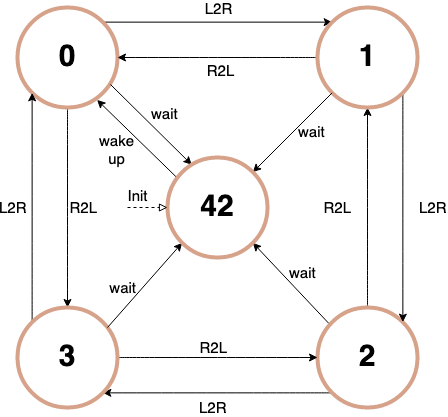
\includegraphics[width=0.4\textwidth]{img/Zustandsdiagramm.png}
		\captionsetup{labelformat=empty}
		\caption{Zustandsdiagramm des Systems\\
		L2R - Left To Right Swipe, R2L - Right To Left Swipe}
	\end{figure}\\
	Auf diesem Bild ist zu sehen wie die 5 unterschiedlichen Seiten des Spiegels mittels den Gesten swipe Links nach Rechts oder swipe Rechts nach Links erreicht werden können.
	Diese beiden Gesten stellten für die grundsätzliche Bedienung die schönste Möglichkeit dar, den Spiegel zu bedienen. Zusätzlich können die Bewegungen swipe Hoch und swipe Runter für erweiterte Funktionalitäten wie Bildschirmhelligkeit oder Ähnliches genutzt werden.
	
	\subsection{Erstellen der Informationsarchitektur}
	Begonnen wurde die Gestaltung der Informationsarchitektur mittels eines \href{https://trello.com/b/hdf8bWp2/sippin-on-my-lean-ux}{Trello-Boards}. Dabei wurden erst auf basis von Nutzer Feedback eine Sammlung an intressanten Features erstellt. Daraufhin wurde mittels \href{https://www.optimalworkshop.com/optimalsort/}{Optimal Workshop} und Card Sorting analysiert wie Nutzer Informationen und Features gruppieren würden. Das gab ein klares Bild über die Struktur der Informationen am Spiegel.
	\begin{figure}[h!]
		\centering
		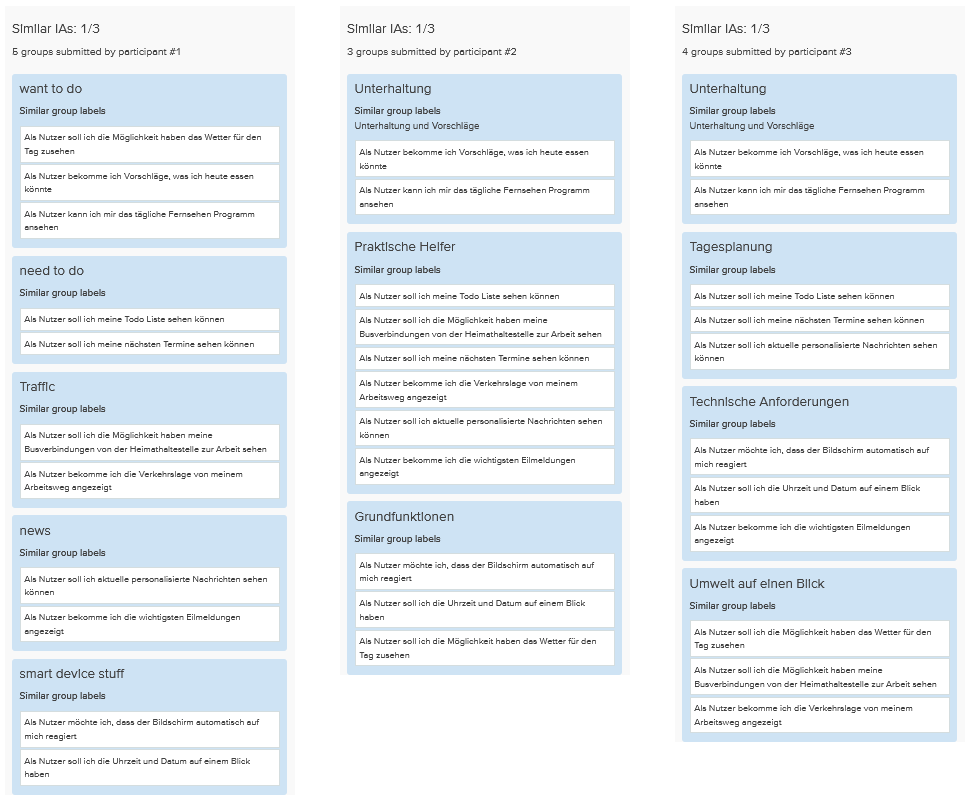
\includegraphics[width=\textwidth]{img/IA.png}
		\captionsetup{labelformat=empty}
		\caption{Informationarchitecture}
	\end{figure}
	\newpage
	Nachdem die Gruppen festgelegt wurden, zeichnete sich ein klares Bild ab, welche Features wie am Spiegel angezeigt werden solle:
	\begin{itemize}
		\item HomeScreen
		\begin{itemize}
			\item Uhrzeit
			\item Datum
		\end{itemize}
	\item Termine \& ToDo
	\begin{itemize}
		\item Termine für heute
		\item ToDo-Liste für heute
	\end{itemize}
	\item  ÖPNV
	\begin{itemize}
		\item Die Abfahrtszeiten vom aktuellen Standort zu einem festlegbaren Ort
	\end{itemize}
	\item  Verkehrslage
	\begin{itemize}
		\item Der aktuelle Weg zur Arbeit samt Stauinformation
	\end{itemize}
	\item Speißeplan
	\begin{itemize}
		\item Die Gerichte des heutige Tages
	\end{itemize}
	\end{itemize}
	
	
	\subsection{Spezifikation des UI}
	Die Entwicklung der UI begann mit Paper Prototyping. Hierbei wurden die ersten ersten Entwürfe auf basis der im vorherigen Schritt erstellten Informationsarchitektur erstellt.
	\begin{figure}[h!]
		\centering
		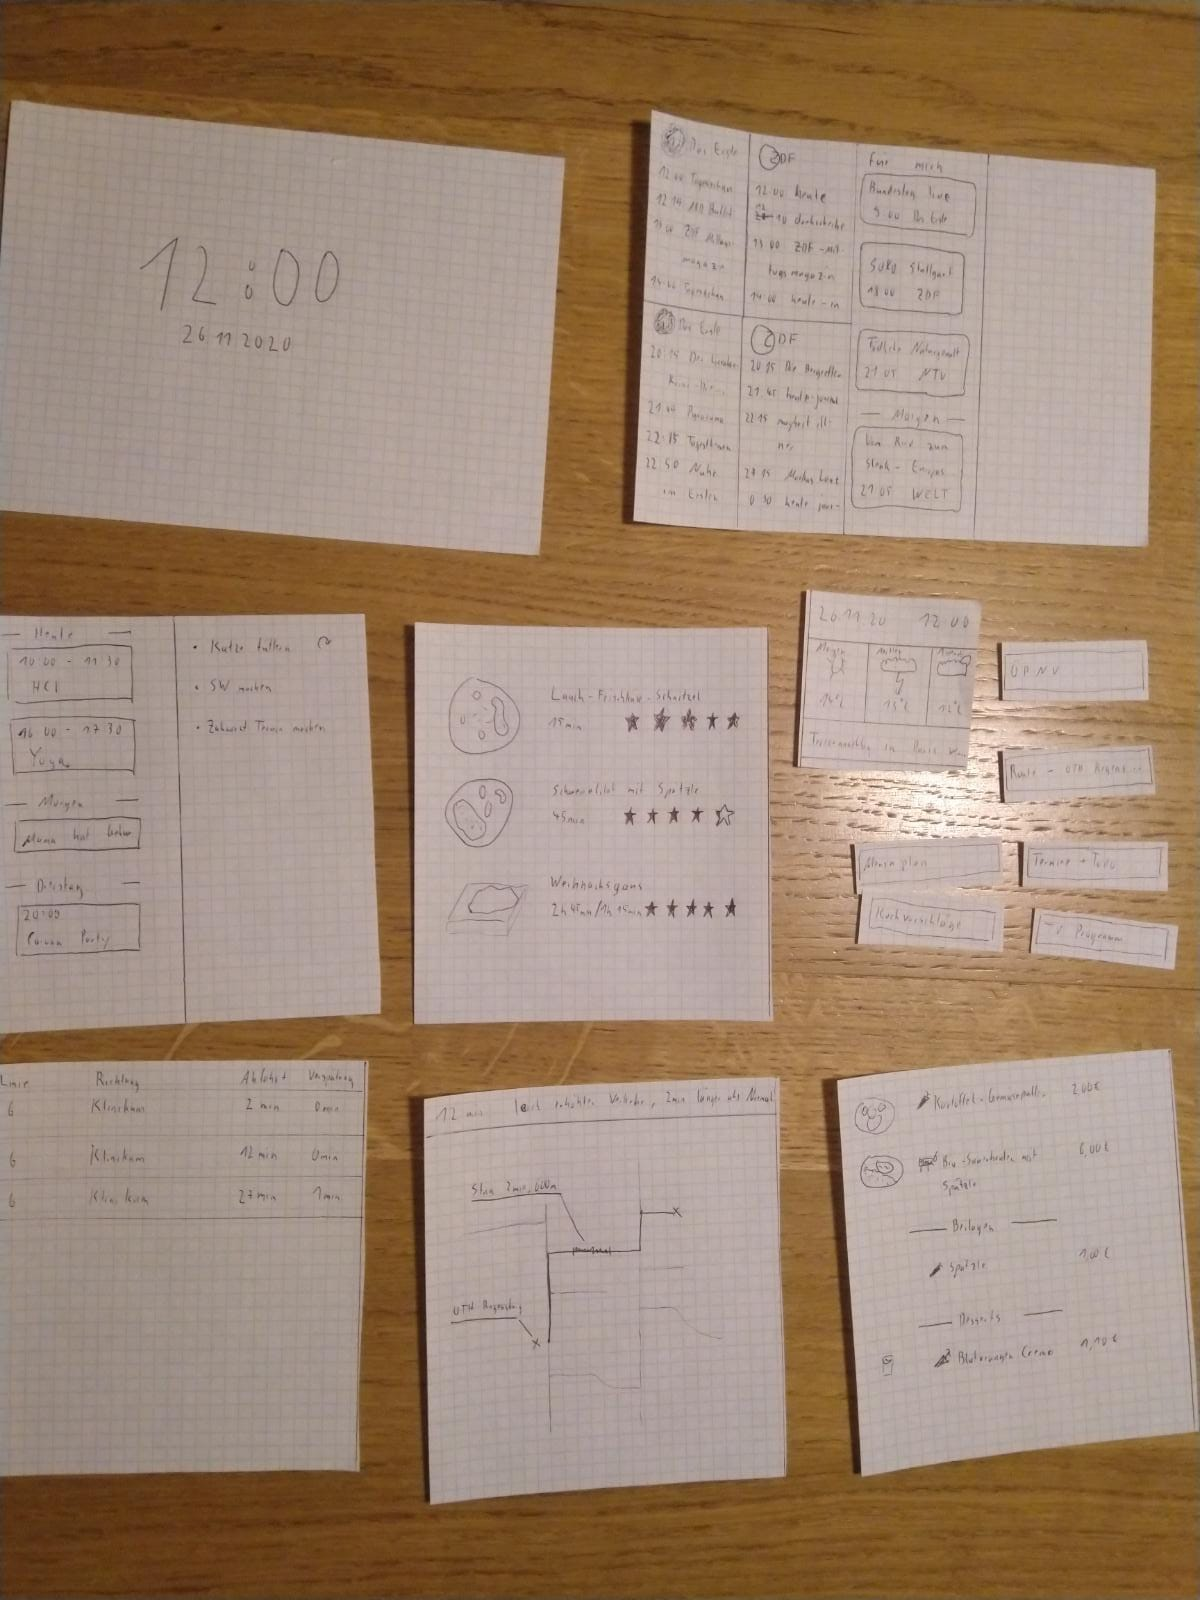
\includegraphics[width = 0.3\textwidth]{img/paperSketching.jpg}
		\captionsetup{labelformat=empty}
		\caption{Paper sketching}
	\end{figure}\\
	Danach ging es weiter mit dem Design der unterschiedlichen Seiten mittels Powerpoint. Hier wurden konkrete Designs mit den verschiedensten UI Elementen ausgearbeitet.
	
	\begin{figure}[h!]
		\begin{subfigure}{0.5\textwidth}
			\centering
			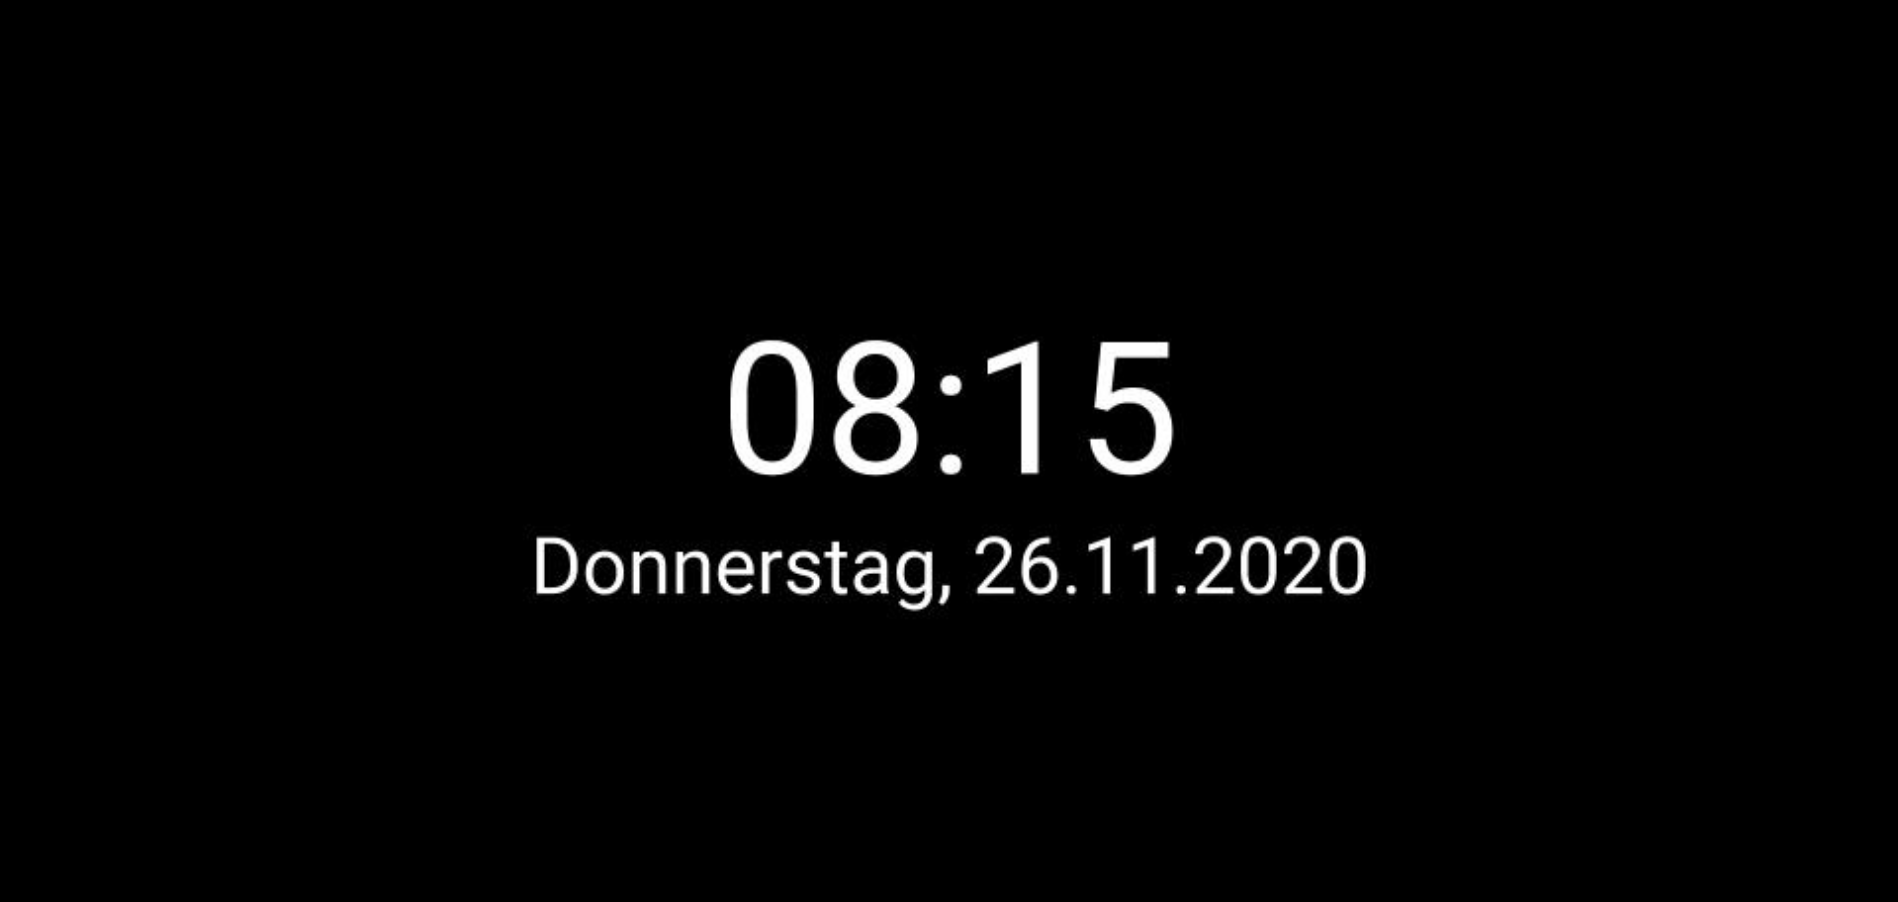
\includegraphics[width = 0.8\linewidth]{img/standby.png}
		\end{subfigure}
	\begin{subfigure}{0.5\textwidth}
	\centering
	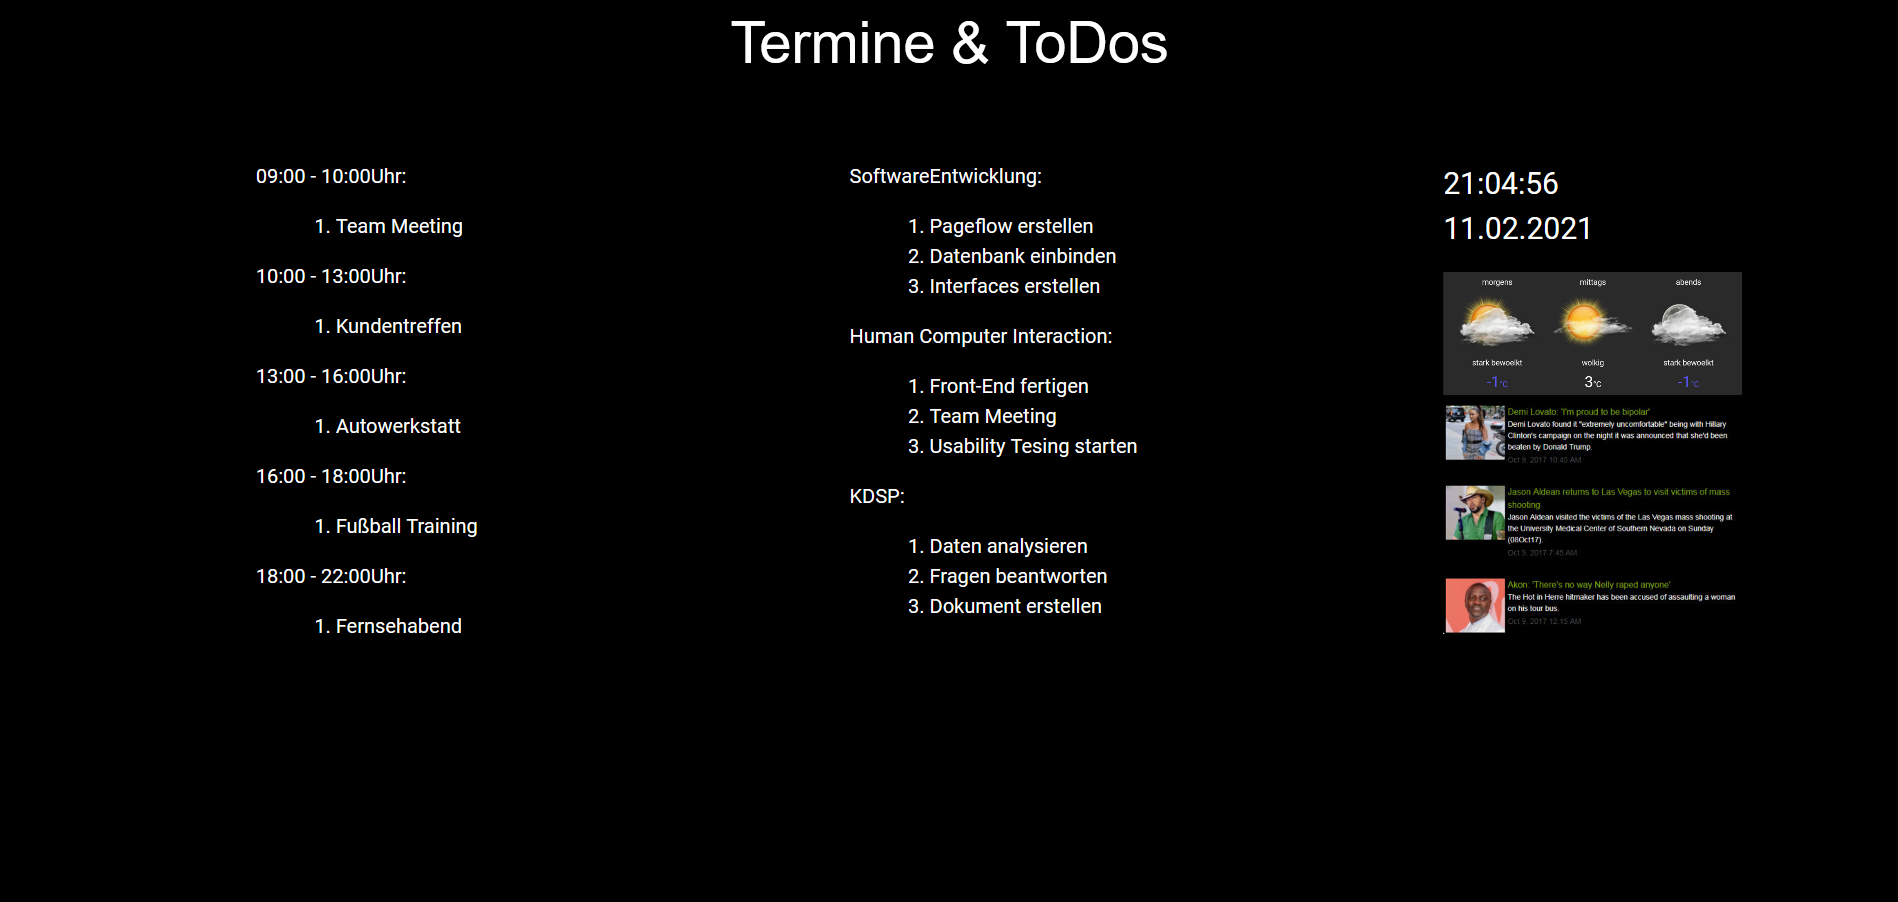
\includegraphics[width = 0.8\linewidth]{img/TermineToDo.png}
	\end{subfigure}
	\end{figure}	\begin{figure}[h!]
	\begin{subfigure}{0.5\textwidth}
		\centering
		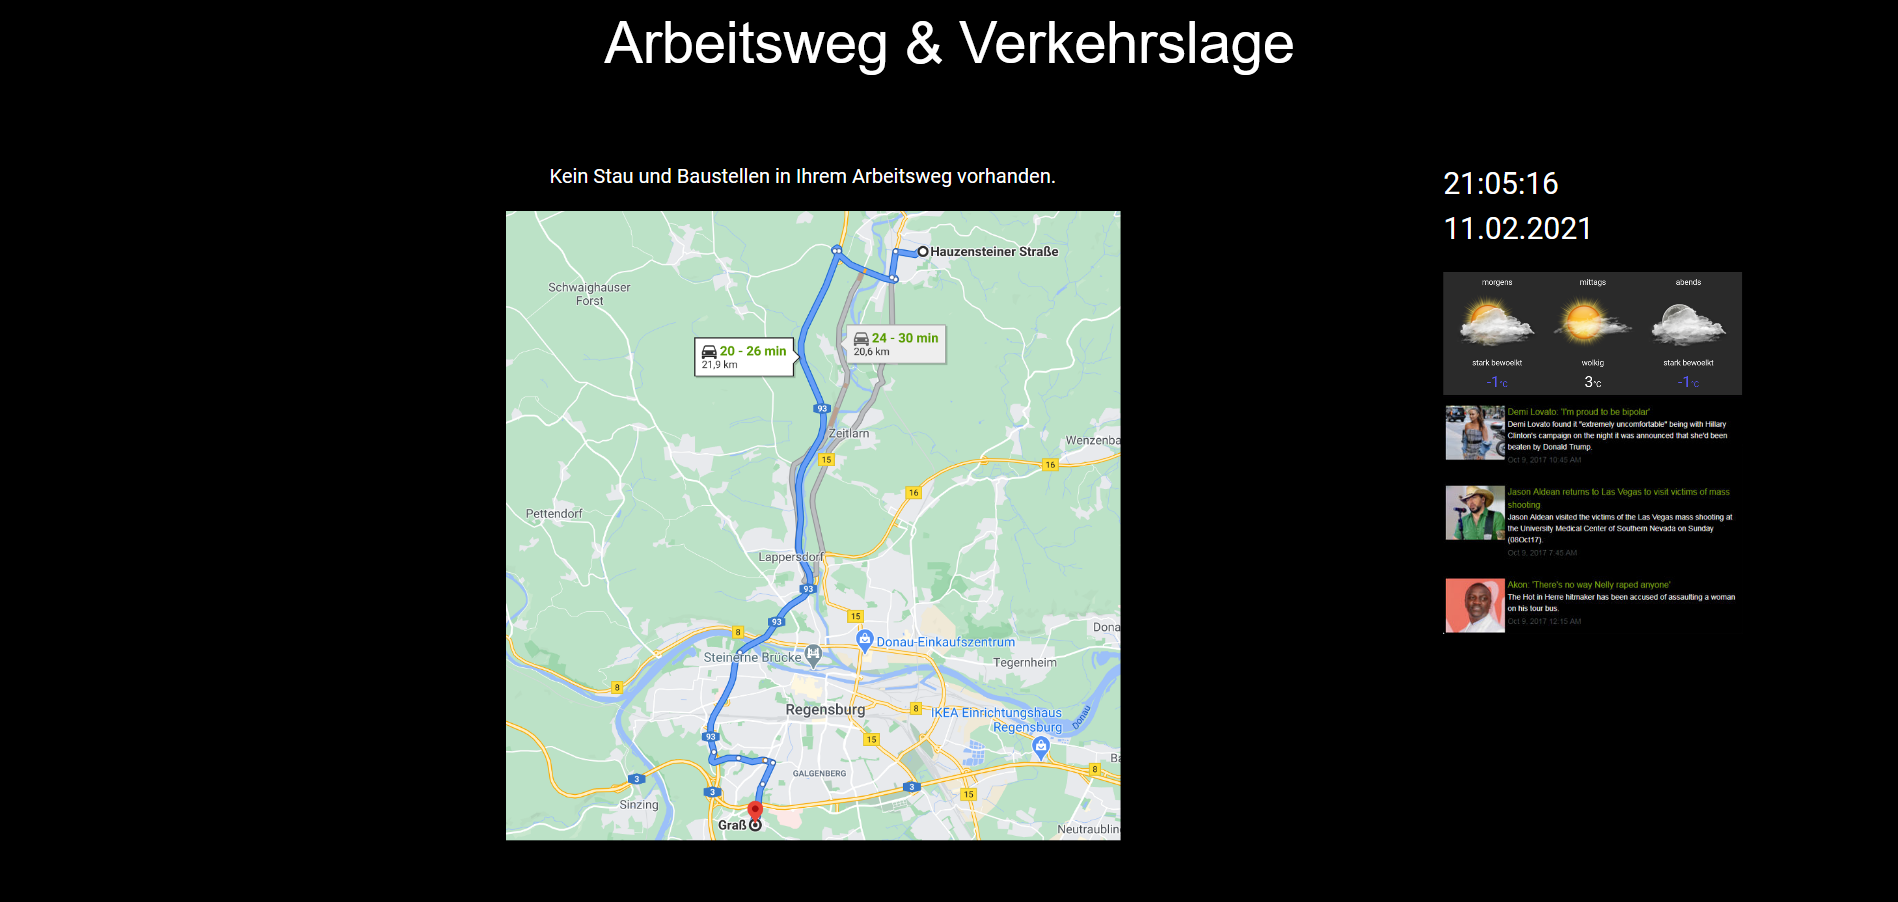
\includegraphics[width = 0.8\linewidth]{img/Arbeitsweg.png}
	\end{subfigure}
	\begin{subfigure}{0.5\textwidth}
		\centering
		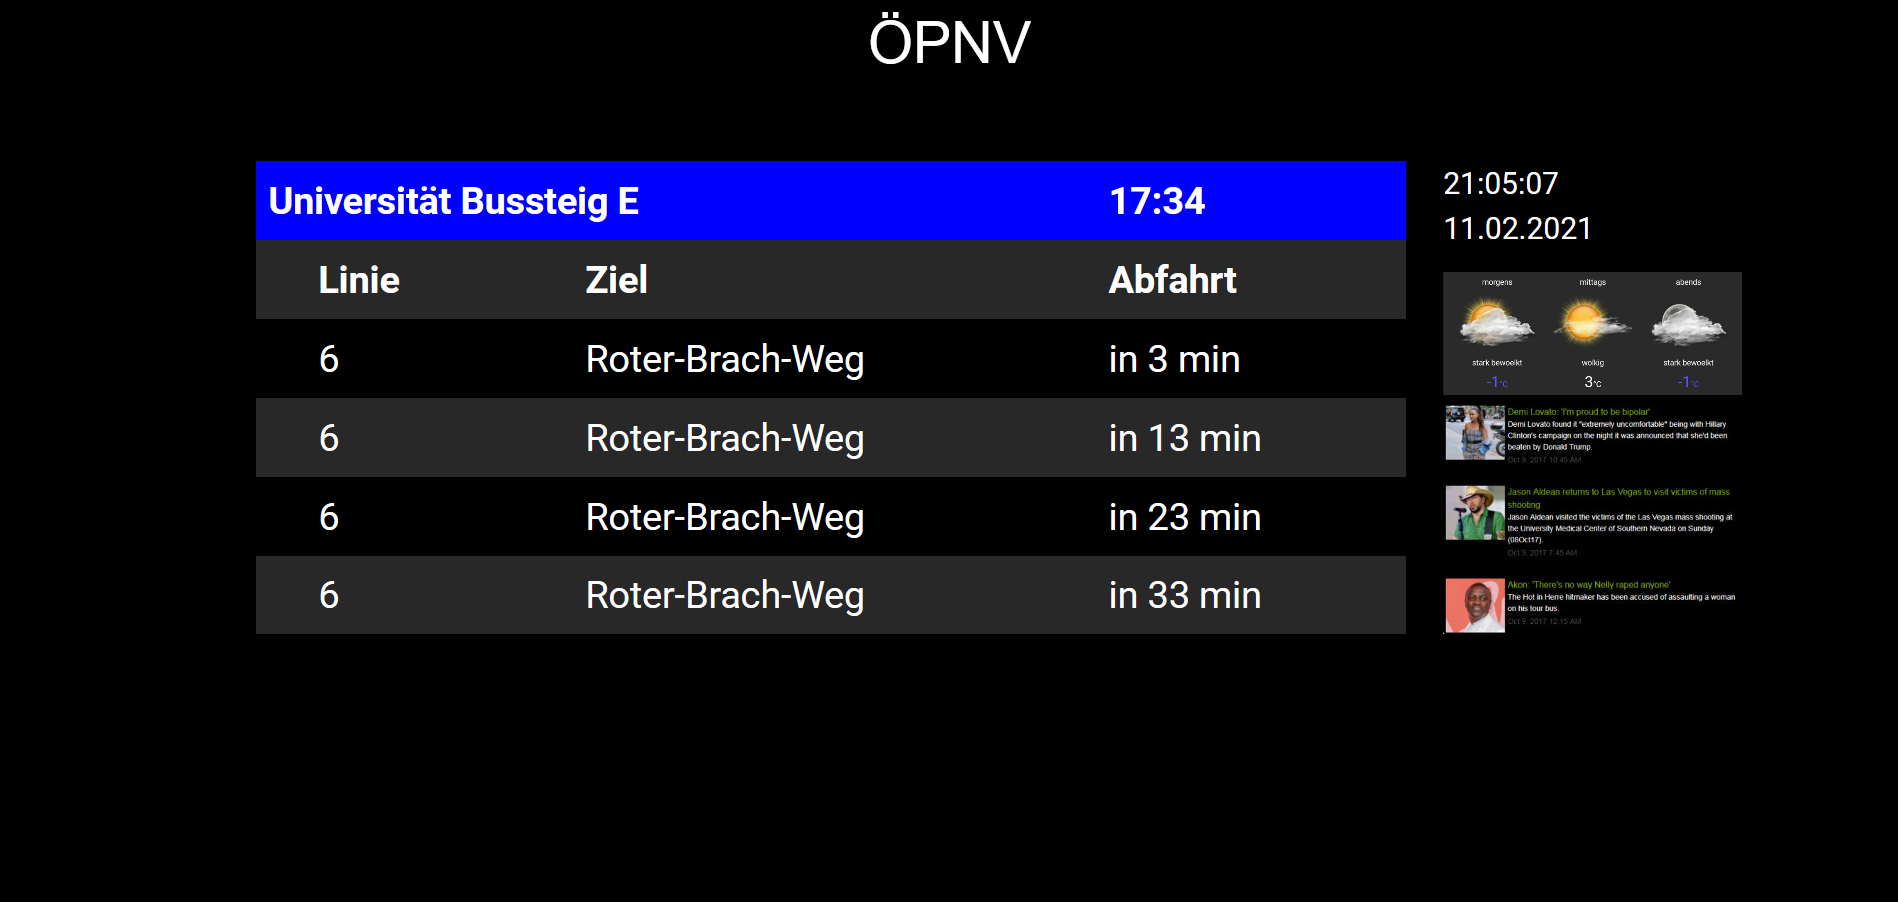
\includegraphics[width = 0.8\linewidth]{img/bus.png}
	\end{subfigure}
	\end{figure}	
	\begin{figure}[h!]
		\centering
		\includegraphics[width = 0.4\linewidth]{img/mensa.png}
	\end{figure}

	\subsection{Prototyping}
	Der Prototyp wurde mittels dem Frontend Framework vue.js und node.js als Backend entwickelt. Dabei wurden die einzelnen Seiten auf Basis der Powerpoint Designs in html Nachprogrammiert. Zur Steuerung des Spiegels wurde ein Leap Motion Sensor mittels des bereitgestellten JS SDKs in den node Server integriert. Darin wurde Gestenerkennung implementiert. Die erkannten gesten werden nun mittels Web Sockets an das vue.js Frontend gesendet. Hier wurden die Gesten nun zur Navigation des UIs verwendet.\\
	Aus Usability zwecken wurden zwei Varianten des Gestenerkennungs-Algorithmuses erstellt. Eine Version die die Gesten nach einer bestimmten Distanz auslöst (also mehrfach swipe mit einer Handbewegung möglich) und eine die bei einer Bewegung nur eine Geste erkennt. Nach User Testing stellte sich heraus, dass die zweite Variante deutlich intuitiver für den User ist, da diese immer versuchen, wie am Smartphone, durchgängige Wischgesten zu tätigen.\\
	Am Schluss wurde ein Konzept zur Durchführung von Usability Tests erstellt. Das erstellte Dokument enthält eine kurze Vorstellung des Projektes, Hinweise zum Usability Testing und Aufgaben, die der Teilnehmer am Spiegel durchführen soll. Die Aufgaben behandeln das Navigieren zwischen den Seiten und das Herauslesen von Informationen. Nach Durchführung des Tests sollen in einem offenen Gespräch zusätzliche Informationen gewonnen werden.
	
	
	\subsection{UI Gestaltungsrichtlinien}
	Um für ein vereinheitlichtes Design zu sorgen, wurde immer die gleiche Schriftart und die gleiche Hintergrundfarbe verwendet. Um Inkonsistenzen zu vermeiden, wurden Komponenten, die auf mehreren Seiten auf die gleiche Art und Weise dargestellt werden, als Fragment in die Seiten eingebunden. Das wären unter anderem diese Komponenten: Uhrzeit, Wetter, RSS-Feed
	
	\newpage
	\section{Aufbau Software System}
	\subsection{System}
	Der grundlegende Aufbau der Software des Smart Mirrors besteht aus einem vue.js client und einem node.js Server. Dieses Konzept wurde so gewählt, da das Leap Motion SDK nur auf einem Windows Rechner oder Mac PC ausgeführt werden kann. Der Server wird dabei auf dem Gerät ausgeführt an dem der Leap Motion per USB verbunden ist, um dort die Gesten des Users erkennen zu können. Diese Gesten werden nun mittels Websockets an das vue.js Frontend übertragen. Die Frontend Website wird dabei auf dem Raspberry Pi, welcher im Spiegel verbaut ist, aufgerufen. Somit können die Eingaben die der node.js Server erkannt hat in echtzeit auf das, sich im Spiegel befindende Frontend, übertragen werden.
	\subsection{Frontend}
	Jede Seite wurde mit vue.js implementiert. Vue.js ist ein clientseitiges JavaScript Webframework, womit Single Page Applications und auch Multi-Page-Webseiten erstellt werden können. Dabei besteht jede Seite aus einer “Single File Component”, die in drei Bereichen unterteilt ist. 
	\begin{description}
		\item[Template Bereich] In diesem Bereich wird der HTML Code eingebunden, der zudem auch vue.js spezifische Inhalte enthalten kann um Elemente einzubinden.
		\item[Script Bereich] Im Script Bereich wird die Logik mittels JavaScript oder TypeScript
		implementiert. Zudem kann die root Instanz oder die bereits erstellten
		Komponenten eingebunden werden.
		\item[Style Bereich] Hier werden die CSS Elemente erstellt. Zudem ist es möglich SCSS, SASS
		oder auch PostCSS zu verwenden.
	\end{description}
	Das besondere an vue.js ist auch, dass alles jeweils aus Komponenten besteht, die zusammenhängen. Das hat den erheblichen Vorteil, wartbaren Code zu implementieren und vor allem für eine gute Wiederverwendbarkeit zu sorgen. 
	\subsection{Backend}
	Der Server stellt primär eine Verbindung mit dem LeapMotion her. Ist diese hergestellt, wartet er auf einen sich verbindenden Clienten. Hat sich eine Verbindung zu dem Spiegel aufgebaut kann der LeapMotion damit beginen die Hände des Nutzers zu erkennen
	Inter detektiert der Server über den LeapMotion in einstellbaren Raten die Position der Hände des Nutzers und speichert diese als SwipeObject zur weiteren Verarbeitung in eine Liste. Damit keine winzigen Bewegungen fehlerhaft erkannt werden, gibt es die Option über zwei Variablen bestimmte SwipeObjecte bezüglich ihrer Variable velocity zu filter und so eine leichte Rauschunterdrückung der detektierten Signale zu ermöglichen.
	Nach diesen Schritten muss der Server nur noch differenzieren, welche Geste der Nutzer ausgeführt hat und diese an den Clienten übertragen, der daraufhin seinen Zustand anpasst und den enstprechenden Inhalt anzeigt. 
	\subsubsection*{Gestenerkennung}
	Zur Differenzierung der Gesten haben wir zwei verschiedene Methoden entwickelt und auch an Nutzern getestet, ob es merkbare Unterschiede zwischen den beiden gibt.
	Die Algorithmen funkiernen einerseits auf einem zeitbasiertem und andererseits auf einem ortsbasiertem Entscheidungsmuster.
	
	\newpage
	
	\section{Evaluierung der Gestaltungslösung anhand der Nutzungsanforderung}
	\subsection{Entwicklungsbegleitende Usability-Tests}
	Während den verschiedenen Entwicklungsphasen wurden immer wieder Usability-Test erstellt und durchgeführt, um den aktuellen Entwicklungsstand zu validieren.
	Dies begann damit, dass am Anfang allgemeine Fragebögen für die potentiellen User erstellt wurden, um ein erstes Gefühl für die 						Nutzungsanforderungen zu erlangen. Dieser war wie folgend aufgebaut:
	\begin{description}
		\item[Allgemeine Fragen] \hfill
		 \begin{itemize}
			\setlength{\itemsep}{-0.5em}
			\item Zu welchen Zeiten stehst du am meisten vorm Spiegel?
			\item Was sind die ersten 5 Fragen, die du dir in der Früh stellst?
		\end{itemize}
		\item[Erlebnis Fragen] \hfill
		\begin{itemize}
			\setlength{\itemsep}{-0.5em}
			\item Zu welchen Zeiten stehst du am meisten vorm Spiegel?
			\item Was sind die ersten 5 Fragen, die du dir in der Früh stellst?
		\end{itemize}
		\item[Spezifische Fragen] \hfill
			\begin{itemize}
			\setlength{\itemsep}{-0.5em}
			\item Welche Apps, Webseiten verwendest du am Morgen?
			\item Hast du schonmal einen Smart Mirror verwendet/gesehen?
			\end{itemize}
		\item[Wunsch Fragen] \hfill
			\begin{itemize}
			\setlength{\itemsep}{-0.5em}
			\item Stelle dir vor du hast einen Smart Mirror, wie sieht er aus? was machst du damit?\\
			wie sieht der Smart Mirror 2050 aus?
			\item Was willst du auf dem Smart Mirror machen können?
			\item Was würdest du dir auf dem Smart Mirror alles anzeigen lassen wollen?
			\end{itemize}
	\end{description}
	Nachdem damit das erste Bild über die Interessen des Nutzers entstanden ist, ging es weiter mit dem Prototyping. Nachdem erste Prototypen 				erstellt wurden, wurde wieder ein Testkonzept entworfen, mit dem der entwickelte Prototyp validiert werden konnte. Dies sah wie folgend aus:
	\newpage
	\begin{center}
	\fbox{
		\begin{minipage}{0.85\textwidth}
			\subsubsection*{Smart Mirror Usability Test}
			Dieser Test soll uns helfen, unseren Smart Mirror Prototypen zu verbessern und Probleme zu erkennen. Dir werden im folgenden mehrere Aufgaben 			gestellt, falls du einige davon nicht erledigen kannst, ist das nicht deine Schuld sondern zeigt uns, was am Prototyp noch zu verbessern ist. Zum 	Beispiel dass der Smart Mirror nicht so intuitiv und leicht bedienbar ist, wie wir es gerne hätten.\\
			Es wäre uns eine große Hilfe, wenn du versuchst bei den Aufgaben laut zu denken, also deine Wahrnehmungen und Überlegungen zu schildern. So 			können wir einen besseren Einblick in die Benutzererfahrung erlangen.\\
			Bitte versuche dich an folgenden Aufgaben in dieser Reihenfolge:
			\begin{itemize}
				\setlength{\itemsep}{-0.5em}
				\item Was siehst du hier?
				\item Versuche den Spiegel zu bedienen
				\item rufe die Termin Übersicht auf
				\item navigiere zur ÖPNV  Übersicht
				\item mache dich mit den verschiedenen Seiten vertraut
				\item navigiere zurück zur Terminübersicht
				\item navigiere zum Mensaplan
				\item navigiere zur ÖPNV  Übersicht
				\item finde heraus, was heute für dich das günstigste Gericht in der Mensa ist
				\item Offener Teil/Fragen nach der Meinung des Users
			\end{itemize}
	\end{minipage}}
\end{center}
	
	\subsection{Evaluierungen}
	Die Evaluierung dient der Feststellung der Erfüllung der Nutzungsanforderungen. Zur Durchführung der Evaluierung wurde am 06.01.2021 ein Konzept entworfen. Ein einseitiges Dokument wurde erstellt, dass dem Probanden vorgelegt werden kann und ihn bei der Durchführung des Tests leitet. Neben allgemeinen Informationen zum Projekt und zum Usability-Test enthält Aufgaben, die der Proband am Smart Mirror durchführen soll. Nachdem der Proband sich an allen Aufgaben versucht hat, sollen in einem offenen Gespräch weitere Informationen gewonnen werden. Jedes der Teammitglieder führte im Laufe der folgenden Wochen je 2 Evaluierungen mit Bekannten durch.\\
	Die Aufgaben sind so gestellt, dass der Proband mehrfach zwischen Screens wechseln muss. Aus den Screens soll der Proband verschiedene Informationen auslesen. Der Fokus der Quantitativen Evaluierung lag auf folgenden Fragen:\\
	\begin{tabularx}{0.95\textwidth}{|X|X|}
		\hline
		\textcolor{tumbleweed}{\underline{\textbf{Frage}}} & \textcolor{tumbleweed}{\underline{\textbf{Antwort}}}\\
		\hline
		Wie schnell kann ein User entdecken, dass durch Swipen die Ansicht gewechselt werden kann? & 2 von 8 Probanden benötigten nach 3 min weitere Hinweise. Die übrigen benötigten durchschnittlich 40 Sekunden.\\
		\hline
		Wie zuverlässig funktioniert die Gestenerkennung?&Nach einer kurzen Eingewöhnungsphase von ca. 3-5 Swipes können User zuverlässig die gewünschten Gesten ausführen. Sehr vereinzelt kommt es auch danach zu falsch erkannten Gesten.\\
		\hline
		Erkennt der User, dass die Screens zyklisch angeordnet sind? Zum Beispiel die Erkenntnis, dass von Screen vier direkt zu Screen eins navigiert werden kann.&Einer von 8 Usern wählten bei der Navigation durch die Screens wiederholt suboptimale Routen, die bei einer rein sequentiellen Anordnung sinnvoll wären\\
		\hline
		Ist die Schrift gut lesbar?&
		Alle Usern konnten die Schrift gut lesen\\
		\hline
		Gibt es Probleme beim Verständnis der gezeigten Inhalte? & Alle User konnten die gezeigten Inhalte versehen\\
		\hline
	\end{tabularx}
		
	\newpage
	
	\section{Arbeitsaufteilung}
	\subsection*{Projektplanung}
	\begin{tabularx}{0.95\textwidth}{|l|X|}
		\hline
		Team & Aussuchen der Bauteile\\
		\hline
		Patrick Gruber & Erstellen der Kostenaufstellung\\
		\hline
		Tobias Gubo & \\
		\hline
		Michael Lazik & \\
		\hline
		Marcus Müller & \\
		\hline
	\end{tabularx}
	
	\subsection*{Verstehen und Festlegen des Nutzungskontexts}
	\begin{tabularx}{0.95\textwidth}{|l|X|}
		\hline
		Team & \begin{itemize}
			\setlength{\itemsep}{-0.5em}
			\item Erstellen des Trello-Boards
			\item Erstellung von UserStories
			\item Konzipierung Interviews
			\item Durchführung Interviews 
		\end{itemize}\\
		\hline
		Patrick Gruber & \\
		\hline
		Tobias Gubo & \\
		\hline
		Michael Lazik & \\
		\hline
		Marcus Müller & \\
		\hline
	\end{tabularx}

	\subsection*{Erarbeitung von Gestaltungslösungen zur Erfüllung des Nutzungskontexts}
	\begin{tabularx}{0.95\textwidth}{|l|X|}
		\hline
		Team & \begin{itemize}
			\setlength{\itemsep}{-0.6em}
			\item  Validierung der Interaktionsmöglichkeiten
			\item  Entwurf der Navigations zwischen den Seiten
			\item Durchführen des Card-Sortings
			\item Paper Prototyping
			\item Erstellung eines Konzepts zur Durchführung von Usability Tests am Prototypen
		\end{itemize}\\
		\hline
		Patrick Gruber & \\
		\hline
		Tobias Gubo &  \\
		\hline
		Michael Lazik &  \\
		\hline
		Marcus Müller & \\
		\hline
	\end{tabularx}

	\subsection*{Aufbau Software System}
	\begin{tabularx}{0.95\textwidth}{|l|X|}
		\hline
		Team & \\
		\hline
		Patrick Gruber & 
		\begin{itemize}
			\setlength{\itemsep}{-0.6em}
			\item Implementierung der Gestenerkennung
			\item Zusammenbau des Spiegels
		\end{itemize}\\
		\hline
		Tobias Gubo & \begin{itemize}
			\setlength{\itemsep}{-0.6em}
			\item Prototyping Setup vo vue.JS und node.JS einrichten
			\item Implemetierung der Socket Kommunikation
			\item Implemetierung der Gestenerkennung
		\end{itemize}\\
		\hline
		Michael Lazik & \begin{itemize}
			\setlength{\itemsep}{-0.6em}
			\item Implementierung der Spiegel UI mittels vue.JS
		\end{itemize}\\
		\hline
		Marcus Müller & \begin{itemize}
			\setlength{\itemsep}{-0.6em}
			\item Debugging-Interface 
		\end{itemize} \\
		\hline
	\end{tabularx}

	\subsection*{Evaluierung der Gestaltungslösung anhand der Nutzungsanforderung}
	\begin{tabularx}{0.95\textwidth}{|l|X|}
		\hline
		Team & \begin{itemize}
			\item Erstellen der Fragebögen
			\item Befragung der Probanden
			\item Erstellen eines Evaluierungskonzept für den Prototypen
			\item Durchführung der Evaluierung 
		\end{itemize}\\
		\hline
		Patrick Gruber & \\
		\hline
		Tobias Gubo & \\
		\hline
		Michael Lazik & \\
		\hline
		Marcus Müller & \\
		\hline
	\end{tabularx}
	
\end{document}